\documentclass[../../main.tex]{subfiles}

% Uses images 218, 220

\begin{document}

\newchapter{Project Review}{project-review}

\section{Design and manufacture} \label{sec:project-review:design-and-manufacture}

\importimage{puc-printed}{PUC, printed in SLS nylon.}{SLS nylon PUC}{0.5}  % TODO: reposition

The assessment of the influence which different power unit layouts have of the vehicle efficiency involves a great magnitude of variables, especially when the test is carried on the same vehicle as in the case of ELMO UAV.
Each configuration requires different specifications in order to be mounted and effects the behaviour of the aircraft in different manners.
A pusher mounted motor, as an example, will have the tendency to increase the wing twist behaviour due to the additional weight on the trailing edge of the wing.
Furthermore, for the cases of a tail or nose mounted units, the tail surfaces will be influenced since they are positioned in the flow field of these.
These are all factors that have a potential influence on the UAV’s efficiency.
Hence, in order to have accurate estimates on the influence of the propulsion location on performance multiple vehicles would have to be designed.
Each one exploiting the advantages of each configuration. 

Due to the time and budget constraints, only one UAV could be built for this project.
Hence the team opted for a simple design which could accommodate all the possible layouts at the expense of efficiency.
The focus was set on obtaining a neutral platform characterized by a constant weight and centre of gravity.
Any increase in cross sectional area caused by mounting structures or aerodynamic effect was considered to be part of the influences induced by the power unit layouts. 

Due to the outbreak of COVID-19 the team was not able to carry out the flight tests planned.
Hence, the absence of the data necessary to compare the effects of each propulsion layout on the UAV performance.
Despite of that, throughout the design and development of ELMO UAV, the impact of each propulsion configuration on the aircraft design was assessed.
The final model does not represent the optimal design for efficiency instead, perhaps, is the conjuncture of all the compromises demanded to ensure the airworthiness of the UAV when flown in any layout. 

As previously discussed, the layout of power unit utilized exhibited great influence on the centre of gravity position as well as the overall weight.
The configurations which offered the lightest model are the fuselage mounted power units.
These do not require additional elements from motor, battery and ESC since the housings were integrated in the nose and tail designs.
Thanks to the positioning of the battery and ESC in the front section of the fuselage, the nose mounted power unit layout presents as positive influence over the CG position by moving it forward to 40\% chord length.
Such positive effect is reduced when for the same battery and ESC position the motor is located on the tail.
This resulted in a shift in CG to 60\% chord length.
A single engine layout, although lighter, demands more reliable components due to the absence of a second propulsion unit in case of engine failure.
Furthermore, for the case of a tail mounted motor, there is the risk of the propeller striking the runway during take-off or landing.
Thus, the addition of a lower vertical stabilizer equipped with a tip bumper in order to ensure a propeller strike. 

For any wing layout additional components (Power Unit Cell) are demanded in order to be mounted.
In addition to this, the use of two power units leads to a larger increase in weight compared to a single motor configuration.
Moreover, the roll rate of the UAV is dependent on the location of the power unit along the wingspan.
For this reason, the ailerons have been sized for a tip mounted motor layout.
The propulsion unit position also influences the design of the wing structure.
The bending moment induced by the wing motor configuration closest to the fuselage is much smaller in magnitude than the tip configuration.
Thus, the need for a stiffer wing structure despite being heavier.
The presence of the 3D printed inserts for the mid-wingspan configurations led to the need of redesigning the flaps.
These had to be split causing a reduction in efficiency.
Thus, the need to increase the flaps’ chord length in order to achieve the CLmax required for take-off. 

The rudder was subject to a resizing process in order to ensure the airworthiness of the UAV when in tip PU configuration.
A motor failure in such configuration would lead to a large yaw moment induced by the large moment arm.
Thus, the increase in the rudder size.
It was then established to be coupled with a nose configuration so to reduce the yawing moment in the case of motor failure.
This although led to a further increase in weight caused by the addition of a third motor unit.
Despite this increase, the overall weight remained below the set limit of 7kg. 

The main difference exhibited between tractor and pusher configurations is the shift in centre of gravity.
This results to move backwards for a pusher configuration respect to its position at 53\% in the case of a tractor configuration.

\section{Testing and Evaluation} \label{sec:project-review:testing-and-evaluation}

% TODO: check captions for this chapter

As it can be seen in Fig. xx, there is a significant difference in weight between configurations.
The use of ballast to maintain constant weight was established.
Doing so, the results gathered from the flight tests would not be biased by the weight differences.
Furthermore, the position of the ballast along the fuselage was dictated by the centre of gravity position for each layout.
In Fig. xx the shift in CG without the influence of ballast can be seen.
The wing tip pusher and nose mounted motor was set to be the weight and CG position baseline.
This decision was taken since this last is the heaviest configuration presenting the most rearwards centre of gravity. 

\importimage{layout-variations}{CG and mass change for each layout, not accounting for ballast; standard configuration is marked in red.}{Variation between configurations}{0.9}
\importimage{flight-test-plan}{flight test plan, listing all configurations which would be tested.}{Flight test plan}{0.9}

\subsection{Flight test} \label{sec:project-review:testing-and-evaluation:flight-test}

Figure showing the abbreviations for each power unit position on the UAV, and a diagram showing the planform of the UAV with each power unit location labelled. 

\importimage{puc-locations}{enumeration of all possible power unit positions on the UAV.}{PUC positions}{0.9}

This table shows all possible configurations of power unit locations with each side of the table as each side of the wing, except for D and E which are the fuselage locations.
Blue shows where both wing have the same configuration and so data can be recorded for that overall layout during a flight with that configuration, green is the initial configurations that would be tested in a knockout format in order to minimise the number of flights required to find the best configuration with the D and E calls as green/blue because they are in both, red is repeats of the lower half of the matrix, and black is for impossible configurations due to both being fuselage locations.
It should be noted that D and E cannot be doubled up either, so where D is on both wings, that is a configuration of only one motor on the nose and the same for E.
There are however configurations where a fuselage motor is combined with a wing motor, this would create an unstable aircraft so in these cases the wing motor would be applied to both wings and the UAV would be flown with three motors, the fuselage motor acting as a safety backup in the case of a wing motor failing.

\importimage{knockout-table}{knockout table for determining the best configuration with minimal runs.}{Knockout table}{0.8}

This is the knockout table, showing the match ups of wing power unit locations required to find the best location of power unit, however no data for each location would be recorded due to the mixing of configurations, and so an additional flight of the best wing config would be required in order to compare it to the fuselage motor locations, totalling 12 flights.
Also, any flights where the distance along the span of the wing is different for the two power units would be difficult to give definitive results due to the off centre CofG.
This would induce a rolling moment and so a constant application of ailerons would be needed to counteract this, which would itself induce a small yawing moment.
This would affect the results because the way of finding if one location is better than the other would be the measure the yaw angle in flight, with the more efficient location being on the opposite side to the direction of yaw, and so any influence on the yaw angle coming from the CofG would not help. 

However, if the power unit locations were all flown symmetrically, the aircraft data could be recorded for each one in order to compare post flight, and the differences in power usage at a constant flight velocity would show which location was the most efficient.
Also, only 12 total flights would be needed, as shown in blue on the matrix table, which is the same number of flights as the knockout method, just with a more accurate method of comparison.
This is therefore the method that would have been used for the testing of the UAV had it been possible.  

The process for testing would involve flying one configuration to accumulate the required data, then change the batteries while changing configuration and downloading the data from the Arduino.
The next configuration could then be flown, and the used batteries put on charge.
The order of flights is shown in Figure x. 

\importimage{flight-order}{list of the planned flights, in order, with the configurations and batteries used.}{Flight order}{0.7}

There would be three sets of batteries for the wing motors, and two sets for the fuselage motors, so that multiple flights could be flown while the used batteries are recharging, reducing delays.
The first three flights would be different wing motor configurations, then one of the fuselage motor configurations would be flown to give the wing batteries extra time to charge before three further flights of the wing configurations.
The wing tip configurations would need to be flown with the nose motor in order to have control in a wing tip motor failure situation, and so these would require three batteries to be used, limiting the charge time of the batteries used in the final flight.

%  TODO: describe process for calculating power draw and getting data off Arduino

\subsection{CFD} \label{sec:project-review:testing-and-evaluation:cfd}

Simultaneously to the full scale wind tunnel test, CFD simulations have been used to assess the validity of the airframe of the UAV.
Furthermore the wind tunnel result have provided data to validate the results coming out of the simulations.
The software used for the simulation is Star-CCM by Siemens.
Using a polyhedral mesh with refinement blocks placed in the key areas such as the wing tip and the flaps (Fig. 16) the residuals exhibited from the simulations were in the order of 1E-7.
The turbulence model used for those simulations was the K-epsilon model.
The flow was assumed to be steady and incompressible.
The difference in the results between the wind tunnel tests and the CFD simulations floated around 8\% for both drag and lift loads.
This difference can be attributed to the presence of the struts in during the wind tunnel test (Fig. 17) as well as inaccuracies present in the wind tunnel model.
A minor increase in the difference raised as the angle of attack of the UAV increased; the percentage raised up to 10\% difference.
As the angle of attack increases the adverse pressure gradient on the suction surface of the wing increases as the boundary layer thickness does.
Hence the flow is closer to stall conditions; case in which the turbulence model’s inherent errors might express in a more prominent manner into the results.
Thus the increase in the difference between the results shown in Fig 18. 

\importimage{cfd-mesh}{section view of the polyhedral mesh utilised for CFD simulations.}{CFD mesh}{0.7}

Through the validation of this results the team was then able to analyse the quality of the flow over the final model of the UAV (Fig. 19).
A non-powered version was analysed in flight conditions exhibiting an overall lift of 77N.
Furthermore the take-off conditions were simulated to ensure that the high lift devices were performing as designed.
At take-off speed equal to 13m/s, flaps deployed at 20deg incidence and 5deg angle of attack the UAV achieves the required CLmax for take-off. 

\importimage{empirical-numerical-comparison}{comparison of physical wind tunnel results with numerical CFD results.}{Comparison of methods}{0.9}

Simulating the interaction between the airframe and the flow arriving from the propeller required more computational power due to the use of a rotating reference frame.
This tool allows to recreate the rotation of the propeller by imposing a rotating flow domain within the free moving flow domain.
This method was first verified against the results gathered from the propeller wind tunnel test.
A difference of 10\% was registered from the real results for the case of 15m/s wind speed and 11500rpm; with residuals in the order of 1E-5.
This difference can be attributed, in part, to the inaccuracies present in the CAD model of the propeller due to the lack of accurate data describing the geometry of this last.
Furthermore, a second source of error are, as before mentioned, the inherent approximations of the turbulence model used.
The decision of carrying the simulations with such CAD model is to attribute to the lack of reliable sources providing accurate models or data of the propeller’s geometry.
A simulation recreating the conditions expressed in Propeller-wing interaction for minimum induced loss (Kroo, 1986) where the propeller swirl interacts with a wing section shows an increase in propeller efficiency equal to 8\% which is coherent with the results found in the same paper.

% \importimage{propellor-flow}{propellor flow structure.}{Propellor flow}{0.3}
% \importimage{trailing-edge-flow}{flow quality at the trailing edge during takeoff.}{Trailing edge flow}{0.3}
% \importimage{flap-flow}{flow behaviour with flaps deployed at 30 degrees incidence.}{Flap flow behaviour}{0.3}

\begin{figure}[H]

    \centering
    \begin{subfigure}[b]{0.49\columnwidth}
        \centering
        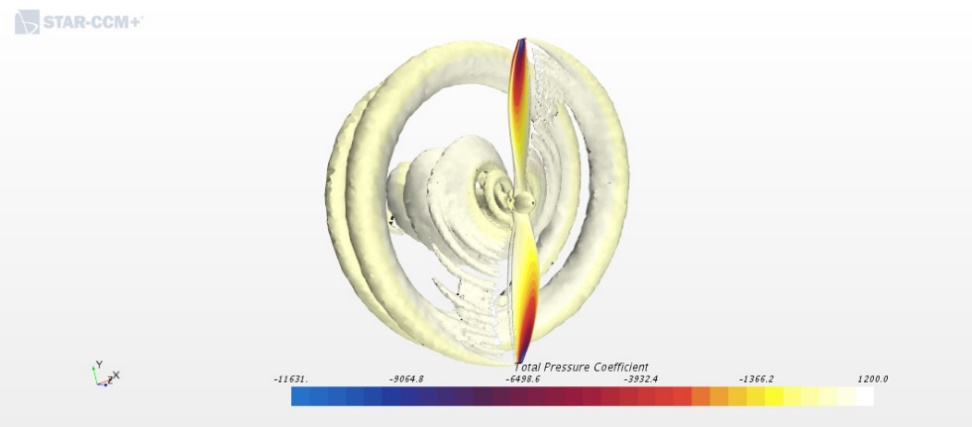
\includegraphics[width=\textwidth]{propellor-flow}
        \caption{Propellor}
        \label{fig:flow-behaviour:propellor}
    \end{subfigure}
    \hfill
    \begin{subfigure}[b]{0.49\columnwidth}
        \centering
        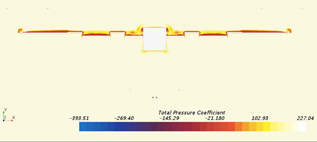
\includegraphics[width=\textwidth]{trailing-edge-flow}
        \caption{Trailing edge}
        \label{fig:flow-behaviour:trailing-edge}
    \end{subfigure}

    \begin{subfigure}[b]{0.49\columnwidth}
        \centering
        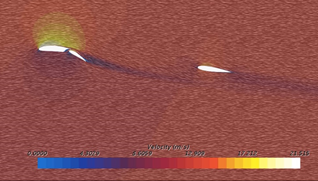
\includegraphics[width=\textwidth]{flap-flow}
        \caption{Flaps}
        \label{fig:flow-behaviour:flaps}
    \end{subfigure}
    
    \caption{results CFD simulations showing flow behaviour at various locations of interest; (c) has flaps deployed at 30 degrees.}
    \label{fig:flow-behaviour}
\end{figure} 

\section{Budget} \label{sec:project-review:budget}

As parts were designed and the construction of the model was established, different elements were added to the budget in order to keep track of costs and maintain the budget.
This included both costs for parts we knew we would need and estimations of costs for parts that were unclear earlier on.
One difficulty we ran into was the cost of 3D printed parts, as the estimations made for the costs of these parts was significantly lower than the final cost.
This was due to the change from PLA to ABS and Nylon construction and also the requirement to use a certain supplier for the 3D printing if it was paid for by the 3D printing fund, which was much more expensive than other suppliers we had originally looked at to budget for the parts.
This meant that at the time of printing (just as the university shutdown happened) the cost  of the 3D printed parts increased massively, and we needed to change the material of a few of the 3D printed parts in order to bring the cost down.
This meant that either the strength of these parts was reduced, or we modified the design in order to accommodate, meaning that the weight would increase, and there was a trade-off here to allow for enough strength while keeping the mass as low as possible.
With a larger budget we would have been able to use more Nylon in the 3D printing and so reduced the mass of the aircraft. 

\importimage{budget}{complete budget table.}{Budget table}{0.9}

The final budget is shown in Figure 85 and it shows costs that happened in black text, and items that were budgeted for but were never bought due to the university shutdown in blue text.
The budget was maximised as much as possible in order to cover the costs of the 3D printing, however the 3D printing budget itself was not fully accounted for, with over £85 remaining, due to the fact that items bought using this budget had to be from a certain supplier which only made parts from Nylon SLS which increased that parts cost by around double for Nylon SLS parts and more for ABS or PLA parts.
This meant that other parts could not be made using this budget as they would go overbudget, and there was no option of supplementing the costs from another part of the funding.
The university funding was fully allocated, with much of the spending being on parts and supplies for the wind tunnel model, with the carbon fibre parts ordered just before the university shutdown while the group still thought that the building of the final flight model would be possible.
The external funding is also fully accounted for, with the parts ordered being the initial purchases for the electronics of the flight model, along with the expendable flight vehicle that was to be used for testing of the avionics and autopilot. 

\section{Impact of Covid-19} \label{sec:project-review:impact-of-covid-19}

\subsection{Progress to March} \label{sec:project-review:impact-of-covid-19:progress-to-march}

By the 13th, the final design was essentially finished and parts were in the process of being ordered, or finalized for being ordered (such as 3D printed or foam cut parts).
The presence and slow effect of the outbreak in the country altered our schedule somewhat, and these would have likely been finished earlier without it.
Initially the group went ahead in the hope that restrictions may be lifted in time to resume construction and testing, so one of the many 3D printed parts was ordered as a test piece, however it soon became clear that lockdown would remain for an extended period of time and we would be unable to build or test our design.
At this point the groups focus shifted onto finalising the design in CAD and mathematically, and surrounding admin work (ensuring budget would still be met despite not being used etc), so that they could be effectively communicated in the project outputs. 

The thin green lines show what had actually been completed relative to our initial timeframe estimates.
As can be seen for some activities, we were behind schedule.
This can be partly attributed to planning, and unforeseen circumstances such as the wind tunnel being fully booked much farther ahead in time than we had planned for, and as such we were thrown off by the fact that we would not be able to begin testing until after Easter.
This widened the range in which we planned to run a physical flight test due to the possibility of needing to fly before wind tunnel tests, which meant we needed to be significantly more confident in the design, as no aspects would have been physically validated beforehand. 

\subsection{Adjustments around restrictions} \label{sec:project-review:impact-of-covid-19:adjustments-around-restrictions}

Once restrictions were put in place, the group quickly shifted to meetings over Skype, and then Microsoft Teams, both as a group and with our supervisors.
These were held mostly held weekly once everyone had settled back into routine, so that communication between ourselves and our supervisors could be maintained.
With regards to the project, the focus quickly shifted from what had been an attempt to build and test, to maximising our efficiency as a group in work on the project outputs, and work quickly began on polishing our CAD and mathematical work (represented by the lines extended beyond the outbreak announcement on the Gantt chart) to be presented in the report, presentation and video, as well as work on preparing for, and then working on these outputs. 

\subsection{Planned future work} \label{sec:project-review:planned-future-work}

The university took the decision to end term a week early, on the 13th of March.
Rates of work had already changed by this point and we were off the original project schedule, as we knew that we would not be building, and as such had the time to refine the mathematical and 3D design to present instead of a physical model and results.  

However, had the COVID-19 outbreak not happened, the project would have looked very different from what it looked like on March the 13th, and what it looks like now.
Observing figure 87, there are two ways to look at what we would have planned to do, which is either based on the original project plan, or what had happened to date.
The thin green lines show what had been completed, and as it can be seen, we were partly behind schedule for some activities (any missing before the purple line are unknown or unimportant to this section).
Had the order to stop not come through, we would have finalised mathematical and CAD aspects of the design by approximately the end of the thin green line for ‘Final model design’, which is where we finished initially, work past that shown in ‘Mathematical analysis’ and ‘CAD design’ are mostly a result of polishing, though a minor change to the tailplane mounting angle (by 0.2 degrees, not significant enough to be a problem) did occur as a result.  

The thin red lines show the teams estimate for what would have occurred had the outbreak not happened based on what had been completed already, and the purple line shows the date of the early end to term.
We had already begun part ordering, and had finalised many of the 3D printed parts, foam cut parts, electronics, avionics and fasteners to order.
Many had been ordered or were prepared to be before it became clear that it would be pointless.
Other parts that were being finalised up to the design finish date would have been ordered as soon as they were ready.  

\importimage{gantt-chart}{initial plan compared with how the project progressed and what would have happened next.}{Gantt chart}{0.9}

The original plan was to have construction and testing complete by Easter and to be making project deliverables over Easter and after to submit by the original deadline.
However, instead we would have been finishing the construction of the UAV over Easter, and have been working on aspects of the report, video and presentation that could have been done, prior to inserting aspects about the final construction and testing into all three.
The team respects that this is off the original plan, and that it would have been more of a ‘crunch time’, however it is felt by all, including our supervisor that it would have been possible, and up to the end we were proceeding as though it would have been; planning new days for wind tunnel testing after Easter, and flight test days with the RC plane group, and our own tests with a Pilot whom we could pay for his services.  

At the start of the project we were made aware of the potential for commercial progression.
Ideally, had the wind tunnel, or flight tests been completed, and results shown that changes were required, these would have been documented and worked upon through analytical processes, CFD, FEA, and iteration in CAD to produce a refined concept of the next UAV.
At the conclusion of design, our budget was projected to be near its limit, therefore we would not have been able to produce a second model based on further design work.
However, had the results and further design work shown enough promise, our team could have worked further with Dr. Kirk to continue the production at a commercial level, with the intention of eventually expanding the scale of the design, or another team could have picked up where our design left off and continued the process of design, testing and refinement on another GDP budget. 

\section{Conclusion} \label{sec:project-review:conclusion}

This project intended to identify the most efficient power unit location on the body of a conventional airframe through the flight testing of a UAV with a movable propulsion unit.
Despite the steady design progress made by all team members, the manufacture and flight testing of the UAV was not possible due to the COVID-19 lockdown restrictions, however, the project was on course to achieve this and complete the desired outcomes.  

The design has been shown to meet the requirements set out by the stakeholder, and the design specification.
The model incorporates reconfigurable propulsion units on the wings and fuselage to allow the testing of multiple propulsion unit locations.
This allows for an informed decision on the most efficient configuration.
An early design was tested both physically in the wind tunnel and mathematically.
The final design was tested in CFD, FEA and mathematically to confirm its airworthiness, allowing for the confidence that the proposed design would be a suitable, stable flight platform for the necessary tests.
The construction of the UAV was planned to be simple to allow for fast changes of the power unit configuration as specified by the hardware requirements. 

Thorough testing of the electrical systems showed that the UAV would be fully controllable by a pilot, whilst recording the necessary data during the flights to determine the most efficient propulsion unit location.
Unfortunately, the autopilot functionality could not be tested due to the lockdown.  

The vision for this project does not end with the conclusion of our allocated GDP time.
The goal of Dr. Ewan Kirk was to obtain a model UAV that would function as a test bed to provide research for future electrical aircraft development.
There is significant work that can be done in the future on this project with the completion of the manufacture and testing of the design laid out in this report, followed by the refinement of a maximum efficiency design based on the results of those tests. 

\end{document}
